\section{Aufbau und Durchführung}

\subsection{Messung des Ausgangssignals}
\subsubsection{Ohne Noise \label{sec:dknoise}}
Zunächst wird der der Versuch entsprechend der Abbildung \ref{fig:Aufbau3} aufgebaut.
\begin{figure}[H]
  \centering
  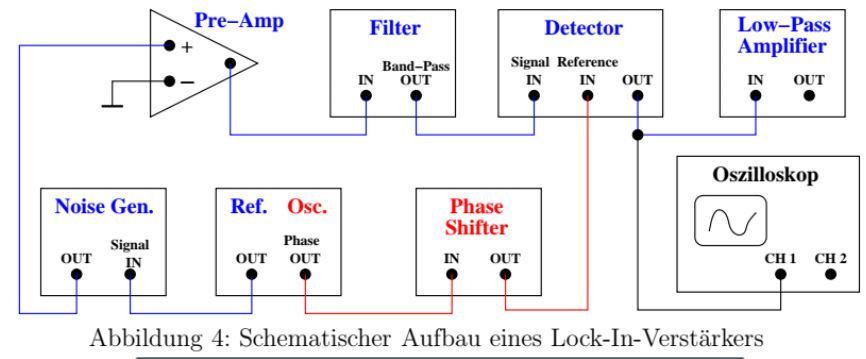
\includegraphics[width=\textwidth]{Text/Bilder/LockIn4.jpg}
  \caption{Schema des experimentellen Aufbaus\cite[4]{sample}}
  \label{fig:Aufbau3}
\end{figure}
Der Noise-Generator wird hier auf OFF gestellt. Daraufhin wird ein
sinusförmiges Signal erzeugt.
Ebenso wird ein Referenzsignal $U_\text{Signal}$ mit selber Frequenz erzeugt. Zur vereinfachten Beobachtung kann das Signal
durch den Gain verstärkt werden.
Sind alle anderen Einstellungen des Lock-In-Verstärkers optimal gewählt, so ist auf dem Oszilloskop
ein Spannungsverlauf ähnlich wie in Abbildung \ref{fig:OUout} zu erkennen.
\begin{figure}[H]
  \centering
  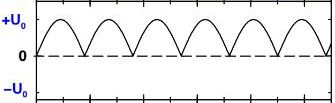
\includegraphics{Text/Bilder/LockIn6.jpg}
  \caption{Ausgangssignal\cite[3]{sample}}
  \label{fig:OUout}
\end{figure}
Der Vorgang wird für 9 weitere Phasenlagen des Referenzsignals wiederholt und die Amplituden der
Spannungen in Abhängigkeit der Phase notiert.
Mindestens 5 Spannungsverläufe, die auf dem Oszilloskop angezeigt werden, sollen gespeichert werden.
Diese wurden jedoch, im Gegensatz zu den Messwerten, vor dem Tiefpassfilter aufgenommen.
\subsubsection{Mit Noise}
Der Aufbau aus \ref{sec:dknoise} wird modizifiert. Nun wird der Noise-Generator eingeschaltet. Dabei soll der Noise
eine ähnliche Größenordnung wie das Signal aufweisen.
Der in \ref{sec:dknoise} durchgeführte Vorgang wird wiederholt, wobei hier die Bilder nicht gespeichert werden müssen.
\subsubsection{LED}
Der Versuchsaubau wird entsprechend der Abbildung \ref{fig:dLED} aufgebaut.
\begin{figure}[H]
  \centering
  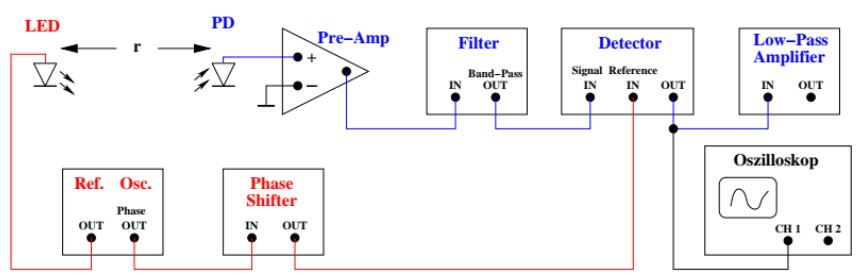
\includegraphics[width=\textwidth]{Text/Bilder/LockIn5.jpg}
  \caption{Schema des experimentellen Aufbaus\cite[5]{sample}}
  \label{fig:dLED}
\end{figure}
Die Leuchtdiode wird eingeschaltet und mit einer Rechteck-Spannung so moduliert, dass sie mit einer Frequenz von
$\SI{50}{Hz}$ bis $\SI{500}{Hz}$ blinkt.
Gegebenenfalls muss das Signal für eine bessere Beobachtung mit einem Gain vergrößert werden.
Ist das Oszilloskop richtig eingestellt, so ist die Spannung am Oszilloskop ablesbar.
Der Abstand zwischen LED und Photo-Detektor wird nun in $\SI{1}{cm}$-Schritten variiert und die Spannungen abgelesen,
bis sich die angezeigte Spannung nicht mehr ändert.
